
\begin{figure}
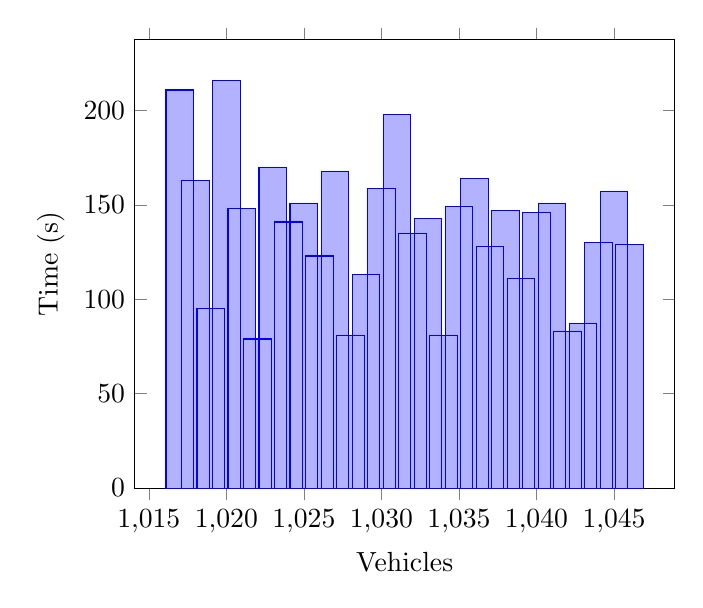
\begin{tikzpicture}
\begin{axis}[
legend style={anchor=west},
xlabel=Vehicles,
ylabel=Time (s),
ymin=0,
ybar,
]
\addplot coordinates {
(1017, 211)
(1028, 81)
(1018, 163)
(1043, 87)
(1042, 83)
(1041, 151)
(1040, 146)
(1046, 129)
(1045, 157)
(1044, 130)
(1019, 95)
(1023, 170)
(1022, 79)
(1032, 135)
(1030, 159)
(1036, 164)
(1037, 128)
(1039, 111)
(1033, 143)
(1031, 198)
(1038, 147)
(1025, 151)
(1024, 141)
(1027, 168)
(1026, 123)
(1021, 148)
(1020, 216)
(1029, 113)
(1034, 81)
(1035, 149)
};

\end{axis}
\end{tikzpicture}
\label{tik:time:100:96}
\caption{100 percent diving with GSC on route $96$}
\end{figure}
